% Section 2: Problem Description & Model
% Compact contributions, expand mathematical model
\begin{block}{\fontsize{46}{54}\selectfont 2. Problem Description \& Model}
    
    {\fontsize{40}{48}\selectfont \textbf{Problem Illustration:}}
    
    \vspace{0.4cm}
    \noindent
    % Two figures side by side: Spatial network | Temporal process
    \begin{minipage}[t]{0.48\linewidth}
        \vspace{0pt}
        \centering
        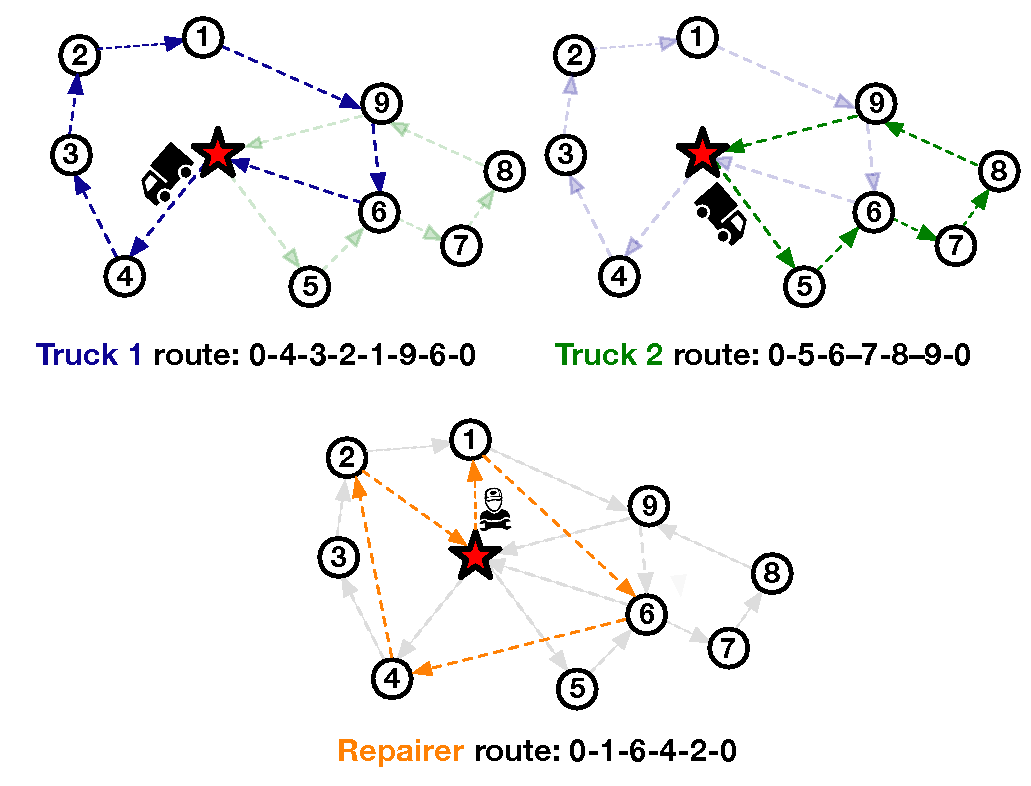
\includegraphics[width=\linewidth,height=26cm,keepaspectratio]{figures/add_repairer.pdf}
        
        \vspace{0.3cm}
        {\fontsize{34}{40}\selectfont \textbf{(a)} Spatial: Network with trucks \& repairers}
    \end{minipage}%
    \hfill
    \begin{minipage}[t]{0.48\linewidth}
        \vspace{0pt}
        \centering
        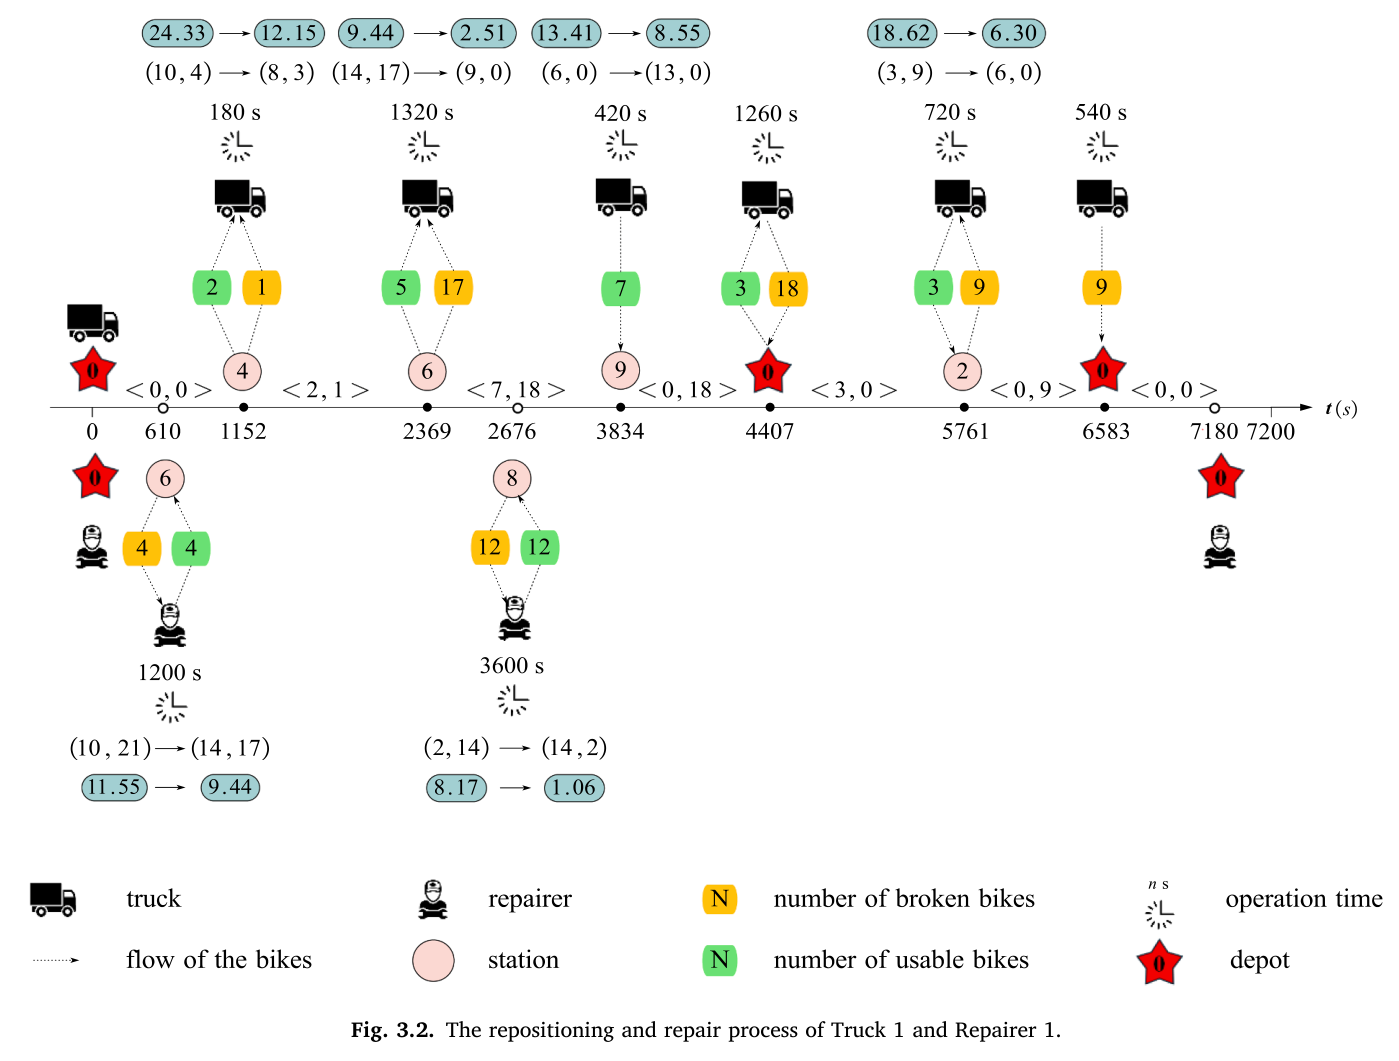
\includegraphics[width=\linewidth,height=26cm,keepaspectratio]{figures/fig_3_2_temporal_illustration.png}
        
        \vspace{0.3cm}
        {\fontsize{34}{40}\selectfont \textbf{(b)} Temporal: Repositioning \& repair process}
    \end{minipage}
    
    \vspace{0.6cm}
    \hrule
    \vspace{0.5cm}
    
    {\fontsize{40}{48}\selectfont \textbf{Mathematical Model (MILP):}}
    
    \vspace{0.4cm}
    {\fontsize{36}{44}\selectfont
    \begin{tabular}{@{}p{0.30\linewidth}p{0.32\linewidth}p{0.34\linewidth}@{}}
        \textbf{Objective:} & \textbf{Key Decision Variables:} & \textbf{Key Constraints:} \\[0.4cm]
        \quad $\bullet$ User dissat. $F_i(\#usable, \#broken)$ & \quad $\bullet$ Routings of trucks \& repairers & \quad $\bullet$ Time budget $T$ for all vehicles \\[0.3cm]
        \quad $\bullet$ CO$_2$ emissions from trucks & \quad $\bullet$ Usable bikes load/unload qty & \quad $\bullet$ Truck capacity (usable + broken) \\[0.3cm]
        & \quad $\bullet$ Broken bikes load/unload/repair qty & \quad $\bullet$ Station inventory balance \\[0.3cm]
        & & \quad $\bullet$ Flow conservation \\
    \end{tabular}}
    
    \vspace{0.6cm}
    \hrule
    \vspace{0.5cm}
    
    {\fontsize{40}{48}\selectfont \textbf{Our Contributions:}}
    
    \vspace{0.5cm}
    \noindent
    \colorbox{HKUGreen!20}{\parbox{0.23\linewidth}{\centering
        \vspace{0.3cm}
        {\fontsize{34}{40}\selectfont \textbf{Novel Problem}}\\[0.25cm]
        {\fontsize{30}{36}\selectfont First to integrate\\on-site repairs}
        \vspace{0.3cm}
    }}%
    \hfill
    \colorbox{AccentGold!25}{\parbox{0.23\linewidth}{\centering
        \vspace{0.3cm}
        {\fontsize{34}{40}\selectfont \textbf{MILP Model}}\\[0.25cm]
        {\fontsize{30}{36}\selectfont Time-indexed\\formulation}
        \vspace{0.3cm}
    }}%
    \hfill
    \colorbox{HKUGreen!20}{\parbox{0.23\linewidth}{\centering
        \vspace{0.3cm}
        {\fontsize{34}{40}\selectfont \textbf{HGS-ADC+SBC}}\\[0.25cm]
        {\fontsize{30}{36}\selectfont Scalable\\algorithm}
        \vspace{0.3cm}
    }}%
    \hfill
    \colorbox{AccentGold!25}{\parbox{0.23\linewidth}{\centering
        \vspace{0.3cm}
        {\fontsize{34}{40}\selectfont \textbf{Insights}}\\[0.25cm]
        {\fontsize{30}{36}\selectfont Cost-effectiveness\\analysis}
        \vspace{0.3cm}
    }}

\end{block}
